%!TEX root = ../thesis.tex

\chapter{Introduction}
\label{chap:intro}

%Ideas->Describing general picture of melodic analysis for description and characterization of IAM. The one we have used in several presentations.
%Ideas-> When you talk about MIR first say what kinds of varied tasks. And then similarity at diff level and pattern recognition has been a focus since a long time! Talk about glass ceiling in similarities, (ref to Joan's thesis). This maybe because similarities has many variablesm and cultural influence is quite recognized one in that. 
%Ideas-> Our ideas behinf using characteristic phrase is like cover song similarity. There is no comparison between two items for similarity. Its from ones mental abstractino or image. See joan's work to get more insights on how has he presented it.
%Ideas-> read some more thesis on this topic and read intros from PR IITB, they are really good points 
%
%
%Overall what all things
%1) What are in generals the problems that world is facing related with digital music
%2) What if machines can understand music like humans do, what can they do
%
%3) MIR dedicated to this kind of research
%4) Varikous topics, variety of problems, basic research, applied reearch, interdesciplinary, mixture of approaches borrowed from other domains, 
%
%
%Joan's approach: Straight starting from task at hand, motivating need for it --> MIR-->

%
%Basically I want to say that data and information is increasing at a fast pace. We ICT tech that can understand, interpret and make sense of digital data like humans do, so that they can make our interaction with the data and information better. So that we can utilize the data and information better in our lives. Many factors play role here, one of them is the cultural and social context. So bsically those factors should also be taken into account. Once these systems learn how to make sense of data, not only will we be able to consume that better but doing this exercise of making machines make sense of the data can also increase our understanding of the concepts surrounding us. This can also enable novel ways od doing stuff, far suprior than what human do for now. 
%
%

%Technologies that can process digital data to understand and interpret it like humans do have becomes nearly a necessity in modern world. Such technology can not only perform tasks that humans already do but can also pave way for novel ways to interact with the data. During the process of developing such technologies we learn and undertand more about the phenomenon in the world. 






\section{Motivation, Context and Relevance}
\label{sec:intro_motivation_context_relevance}

%Repeating structures are important information units in data such as text, DNA sequences, images, videos, speech and music~\citep{Buhler2002b,Herley2006}. Patterns are exploited in a variety of ways, ranging from signal level tasks such as data-compression~\citep{Atallah1999} to more cognitively complex tasks such as analyzing an art work~\citep{van2010texton}. In music domain, identification of repeating structures in a musical piece is fundamental to its analysis, understanding and interpretation~\citep{Cook1987,Lerdahl1983}. 

\subsection{\titlecap{\glsentrylong{mir}}}
\label{sec:intro_motivation_mir}

\Gls{mir} is a growing interdisciplinary research field that primarily addresses topics involved in understanding and modeling of music using information processing methodologies~\citep{roadmap_mir}. In particular, it aims to advance our knowledge in representing, understanding, describing, retrieving and organizing music related data, which opens up wealth of possibilities to develop novel ways to interact with music~\citep{casey2008content,orio2006music,burgoyne2016music}. As mentioned \gls{mir} is interdisciplinary field, which stands at intersection of well established disciplines such as signal processing, pattern recognition, musicology, psychoacoustics, music perception and cognition, information science, and computer science (machine-learning). \TODO{remark that we are mainly talking about content based MIR}

A significant effort in \gls{mir} is dedicated towards automatic description and characterization of music content to extract musically and semantically relevant information. Computational approaches in \gls{mir} for tasks such as melody extraction~\citep{salamon:phd:13}, chord estimation~\citep{mcvicar2014automatic}, music key estimation~\citep{peeters2006chroma}, motif discovery~\citep{collins2011improved,Conklin2010}, music structure analysis~\citep{paulus2010state,serra2012unsupervised}, music similarity~\citep{joan_thesis}, genre classification~\cite{aucouturier2003representing} and emotion recognition~\citep{kim2010music}, tempo and beat tracking~\citep{gouyon2005review,scheirer1998tempo} describe and characterize music pieces in terms of different musical aspects such as melody, rhythm, harmony, structure and emotion. However, the definition, interpretation and relevance of these musical aspects are not universal and vary significantly across different music traditions,  and personal, cultural and social contexts. \TODO{You can add Xavier's sentence on his interpretation of description of MIR systems} Failing to account many of them, a significant number of existing computational approaches in \gls{mir} might be hitting the so-called ``glass ceiling"~\citep{pachet2004improving,casey2008content}. This phenomenon is fairly evident from the slowing rate of improvement of the approaches in \gls{mir} over years, as seen in the results of MIREX\footnote{http://www.music-ir.org/mirex/wiki/MIREX\_HOME} evaluations. There exists a semantic-gap between the automatically extracted music descriptors from audio signals and the high level music concepts that humans relate to~\citep{celma2006foafing,casey2008content}. There is a need to bridge this gap and to take a broader perspective to describe music by also considering the cultural, social and user context into account~\citep{roadmap_mir}. \TODO{highlight lack of knowledge infusion from top dwn. Most approaches work on audio based on features and try to describe higher level concepts}.

\TODO{Bob sturm stuff, rephrase}. In this context, it is worth mentioning the recent debates on whether machines are really understanding or ``making sense" of music or are just producing good classification numbers in evaluations \TODO{ref: bob sturm horse paper}. This skepticism of our interpretation of several \gls{mir} systems become evident when the trained methods for a number of \gls{mir} tasks produce varied results when fed with different inputs that only differ in terms of perceptually or musically inconsequential changes \TODO{Genre + deep net ref}. Whether intelligent machines should learn to perform a computational task similar to how humans do or not is a topic for debate \TODO{ref}. Irrespective of that, the approaches in \gls{mir} should at least scale to the repertoire on which they are developed and should be invariant to trivial low-level changes. The arguments are if these different inputs with trivial differences are fed to the system during the training phase, they can be well handled and learned. Probably true to an extent, but in \gls{mir} its virtually impossible to work with the whole real-world collection of music and most of the test datasets tend to be a small fraction of that. Therefore, robustness to trivial changes might be important to scale the approaches and systems developed in \gls{mir}. Moreover, one of the motivations of several researchers behind developing such systems is to learn more and get novel insights into music and validate our understanding of music, which might be futile if the systems are not really learning the underlying musical concepts. In this dissertation we try to steer away from such pitfalls by laying emphasis on the human interpretability of the research results, and wherever possible, of the output of the intermediate stages of our approaches. We are very aware that human interpretability doesn't guarantee that the approaches are generalizable or scalable, but, at least we are conscious of what our systems are learning, which eventually helps to improve them further. In addition, we work with a diverse, representative and sizable collection of \gls{iam} that contains editorial metadata and other relevant information in addition to the audio recordings, which can be regarded as a representative subset of the real-world audio collection of \gls{iam}~(\chapref{chap:corpus_music_corpora_and_datasets}).

%
%\begin{itemize}
%	\item What is music information retrieval
%	\item What is the context in which music information retrieval is growing
%	\item Why is MIR getting more important and finding many applications
%	\item Successful examples of MIR
%	\item What are the different contexts related with music that MIR can help in
%	\item what more?
%\end{itemize}

\subsection{CompMusic Project}
\label{sec:intro_motivation_compmusic}

Despite great advancements in the field of \gls{mir} in the last two decades, the outcome and generated knowledge to a large extent is not directly applicable to several music cultures of the world. This can be largely attributed to the fact that the research in \gls{mir} has been mainly focused on the western commercial music of the past few decades~\citep{XavierSerra2011}, and therefore, it does not extend to other music traditions. The western commercial music has shaped the undertaken research problems in \gls{mir}, and as a natural consequence, the obtain solutions are best suited for this music repertoire. These solutions often fail to respond to the multicultural reality present in the musics of the world~\citep{XavierSerra2011}. To gain insights on the factors responsible for capping the performance of the current \gls{mir} approaches (\secref{sec:intro_motivation_mir}) and to make the research outcome applicable to different music traditions of the world, development of these approaches in a multicultural context is important. Note that by this we do not imply that research  in \gls{mir} is only focused on western popular music. There has been work done on analysis of flamenco, folk, ethnomusicology, western classical \TODO{rephrase last line and put references}.

CompMusic\footnote{http://compmusic.upf.edu/} (Computational Models for the Discovery of the World'd Music) is a research project funded by the European Research Council that was born from the concerns mentioned above~\citep{XavierSerra2011}. The project focuses on five music traditions of the world: Hindustani (North India), Carnatic (South India), Turkish-makam (Turkey), Arab-Andalusian (Maghreb), and Beijing Opera (China). One of the main objectives of the CompMusic project is to promote and develop multicultural perspectives in \gls{mir}. In particular, the project aims to advance in the automatic description of music within \gls{mir} by identifying musically relevant problems coming from culture-specific contexts and by developing domain specific approaches to solve them. The solutions devised in this project can result in new computational methodologies of interest for a wide variety of music information processing problems. Thus, addressing the research problems in the context of diverse music cultures will not only help in advancing the knowledge in the specific cultures, but also expand the scope of current research in \gls{mir}. Furthermore, it can help bridge the semantic-gap and push the glass-ceiling. \TODO{Something on stress on good data, and how can it improve the systems}

The work presented in this dissertation for description and characterization of melodies in \gls{iam} has been carried out as a part of the CompMusic project and it aligns with the goals of the project. The cultural specificities of \gls{iam} have shaped our research work at each step ranging from the identification of research problems and building the data corpus to the choices made for different procedures and parameter settings. The insights gained during the handling of the challenges posed by the peculiar characteristics of melodies in \gls{iam} (\secref{sec:intro_challenges_oppurtunities}) will help expand the scope of the existing approaches in \gls{mir}. Our work paves the way for cross-cultural studies, which can help us get better insights into the influence of cultural training on perception and cognition of different musical aspects.


%\begin{itemize}
%	\item MIR is important and things are going fine, what's the issue then? Is there any bias in the kind of music tradition being analyzed in MIR right now? whats the reason for this bias
%	\item What kind of music traditions are kind of ignored for anlaysis now?
%	\item What's the reason why no one wants to consider them?
%	\item Is it even relevant to consider them? Which ones amongst them are the easiest ones or the most relevant ones to consider
%	\item Does everyone get benefitted from this kind of work? how things improve overall by doing this?
%	\item What is the objective of COmpMusic project, which music traditions it focuses on. 
%	\item What kind of methodologies are being worked upon in compmusic, What is the main philosophy
%	\item The idea of open-acess and reproducibility
%	\item what more?
%\end{itemize}

\subsection{Description and Characterization of Melodies}
\label{sec:intro_description_characterization_melodies}


\blockcquote{ringer2001melody}{``\textit{Melody, defined as pitched sounds arranged in musical time in accordance with given cultural conventions and constraints, represents a universal human phenomenon traceable to prehistoric times...wherever music became an intrinsic condition of life, certain common melodic procedures were necessarily adopted, because they satisfied basic physiological and biological requirements, if not the aesthetic imagination, per se....`Melodic unity' is configurationally speaking an intrinsic psychoacoustical function of melodic generation in a given historical-cultural context and music in the end be experienced as such...Above all, as a social product, melody is part and parcel of the cultural or subculture to which it owes its existence...}''}

Essentially, there are two points to note here; first, that melody is innate to humans and is one of the fundamental aspects in most music traditions, and second, the perception of melody is shaped by cultural influences. Melody is manifested in a number of phenomena that surround us, for example, in lullabies, nursery rhymes, intonation in languages, and music. Melody also facilitates memorization. Historically, when the printed medium was not prevalent, knowledge was transmitted orally across generations, often set to music to make memorization easier. Even today, as listeners, very often we try to reproduce the melody of the song we want to recall. The importance of melody in our musical experiences makes its analysis an interesting topic of research. With no surprises, a significant part of the efforts in music content processing in \gls{mir} is dedicated to computational analysis of the melodic aspects of music. Such an analysis is even more important for melody dominant music cultures such as \gls{iam} and Flamenco.

The arrangement of the pitched sounds in a melody is shown to be hierarchical in nature\TODO{ref: generative theory}, where the pitched sounds group together into melodic phrases or motifs, which in turn group into sections that together form stanzas finally leading to the musical piece. At each level there is a complex interplay between these different elements of melody. Computational analysis of these melodic elements can provide insights into musical concepts operating at different levels of abstraction and complexity, and eventually help us automatically extract higher level semantic descriptors.

\textquote*[Cambouropoulos2006]{\textit{Music becomes intelligible to a great extent through self-reference, i.e.,~through the relations of new musical passages to previously heard material. Structural repetition and similarity are crucial devices in establishing such relations}}. Repeating structures or patterns in melodies play a pivotal role in organizing an incoming music stream. \textquote[schenker1980harmony]{Only by repetition can a series of tones be characterized as something definite. Only repetition can demarcate a series of tones and its purpose. Repetition thus is the basis of music as an art}. This makes the computational analysis of melodic patterns and motifs a crucial task in the automatic description of melodies, which is also evident from a large number of studies dedicated to this topic. Discovery of repeated melodic patterns within a music piece (often referred to as intra-opus discovery) can help reveal the structure of the piece, and form the basis for studying the stylistic characteristics of an artist. Such repeating patterns when analyzed at a corpus level can not only help establish similarities between different artists and compositions, but also, facilitate studying stylistic influences across them. 

It is worth noting that the idea of repetition as mentioned above refers to a musical repetition, wherein across occurrences the musical unit can undergo a series of transformations. Few examples of such transformations in the case of melodic patterns are pitch transposition, non-linear time-scaling and addition/deletion of melodic ornaments. A computational approach for pattern discovery should be robust to such transformations. Thus, the task of discovering patterns encapsulates the task of computing similarity in music, which is crucial in developing novel methodologies for music recommendation, navigation and music discovery. As mentioned above, the perception of melody is shaped by the cultural influences. The meaning, interpretation, functional role, relevance and manifestation of the elements of melody as discussed above may significantly differ across music cultures. For a holistic understanding of these musical concepts it is important that they are studied within a multicultural context. 

Al the reasons mentioned above motivate us to study computational approaches for the description and characterization of melodies in \gls{iam}. Unavailability or rather inappropriateness of symbolic type music representation, long duration of music performances (sometimes over an hour), distinct melodic characteristics, improvisatory nature of music, and complex melodic framework of \gls{raga} (Section XX) are few peculiar characteristics of \gls{iam} that provide unique opportunities and challenges to expose the shortcomings of the current \gls{mir} systems. Devising novel approaches that overcome these challenges will not only result in making \gls{mir} more accessible to \gls{iam}, but it will also push the boundaries of \gls{mir} technologies. Such computational approaches can enable \gls{raga}-based music retrieval from large audio collections, semantically meaningful music discovery, musically informed navigation and several applications around music pedagogy. In the next section we provide a detailed overview of the challenges and opportunities offered by \gls{iam} in computational analysis of its melodies, which further adds to our motivation behind selecting \gls{iam} for this study.







%
%concept of similaries, and then recommendation and navigation etc
%
%What can we do in practical applications with this this
%
%In the past done this this, since these differ we need to do for indian...
%
%
%These elements, their role, significance and manifestation changes across music cultures. also context changes, many things are diff signal etc...copmlexity is didd. concept of music generation is diff.. improvisation idea is diff...idea of composition is diff
%
%
%
%While a precise objective definition of melody is argued to be impossible (XXX), at a 
%
%Automatic description and characterization of melodies are broad topics with a wide scope that can include a number of computational tasks addressing different aspects of melodies. 
%
%
%Melodies can also be seen as being structured hierarchically according to the melodic framework prevalent in a music tradition. Starting from the basic unit, which is a pitched sound, a note, through a temporal interplay of such events building the whole melody. TYpically arrangement is such that notes group together into phrases, which is a unit that can be considered as a unit incorporating artists thoughts. Silence plays an important role in this structrures and a delimiter. Patterns play an important role in comprehension of melodies and are very important to be studied. It is also linked to lyrics and the strucrture in the lyrics, different lines, stanjas and probably like verses, chorus, which is another hrirarchy of this structure. And then when seen as a whole the fullpiece is basically a piece of art conveying what artist wanted to express and musically is making a unit of a framework (like raga tala). Issue of similarity
%
%Description and characterization are umbrella terms involving a number of computational tasks that act at different levels of abstraction and musical concepts.  Study and analysis of each of these units and different strucrtures at different level is contributing towards description and characterization of melodies. Studing XX is helpgul in XXX and form the basis or input for other tasks. Studying XXX is helpful in blah blah.
%
%
%
%Several different ways to approach description and characterization of music. one of whch is through doing the same for the melody. very widely addressed..
%Automatic analysis for description and characterization of melodies is an imp task, core in mir. examples of the tasks that do that...
%
%Melodies is composed of xxxx, heirarchical arrangement. Tonal and Temporal arramgement. 
%
%One of the ways is pattenr, very imp. 
%
%We can describe at diff level, notes it uses, key and mode, stylistic description, structural description, description of the characterisics
%
%In this thesis focus on patterns. 
%
%what is raga and makam commonly called asd doing that is imp. and why
%
%
%so basically melody is imp, melodic desc is imp, it can help in XXXXXX, it can be at various levels, low level to high level, each one has its own imp, we focus more on patterns, patterns are imp, and why so..then melodic framework, the most abstracted higher level view, we do that too, and since that is closely linked with mood and emotions that directly becomes relevant for recommendation and navigation and those kind of stuff
%
%First time pattern discovery is addressed to this level

description 
\section{Melodic Analysis in Indian Art Music: Challenges and Opportunities}
\label{sec:intro_challenges_oppurtunities}

The current thesis focuses on developing computational approaches for description and characterization of melodies in \gls{iam}. There are ample reasons why such an analysis is relevant for \gls{iam}, and why working on \gls{iam} can help broaden the scope of the current approaches for melody processing in \gls{mir}. In this section we highlight these reasons by presenting the main challenges in the computational melodic analysis of \gls{iam}, and by presenting the new opportunities that it offers. 


One of the challenges in computational analysis of \gls{iam} arises from the fact that symbolic music scores corresponding to music performances are nearly inexistent, and audio recordings are the main data source for computational analysis.  Though, there exists a small repertoire of prescriptive symbolic scores corresponding to musical compositions, the scope and relevance of such music representation in \gls{iam} is practically restricted to its role as a tool for documentation and music training. This is understandable as musical compositions merely act as skeletons in music performances in \gls{iam}, and the essence of the music lies in the improvisatory aspects. In addition, the existing symbolic music representations do not capture the nuances of the melodic material used in the performances of \gls{iam}. \gls{iam} has been transmitted orally across generations and has predominantly followed a tradition of Guru-Shishya parampara (``lineage'' system).  Due to these factors \gls{iam} mainly possesses audio music collections. It is well known in \gls{mir} that computational analysis using audio recordings is challenging as extraction of a reliable melodic representation from audio signals is still an active topic of research. However, at the same time working with the audio music collections of \gls{iam} can be seen as an opportunity.  The extraction of predominant melody in audio recordings of \gls{iam} appears to be relatively easier compared to other music traditions such as rock, jazz and orchestral music. This performance difference is evident from the MIREX results\footnote{\TODO{link?}}. It can be attributed to the fact that a performance of \gls{iam} typically involves a small number of simultaneously playing musical instruments compared to other music traditions, resulting into a sparse polyphonic audio content, which is easier to process for the melody extraction algorithms. In addition, since \gls{iam} is a melody dominant tradition and comprises largely vocal-based music, the lead voice is predominant compared to the accompanying instruments. These factor make the extraction of predominant melody in \gls{iam} relatively easier. 

\begin{figure}
	\begin{center}
		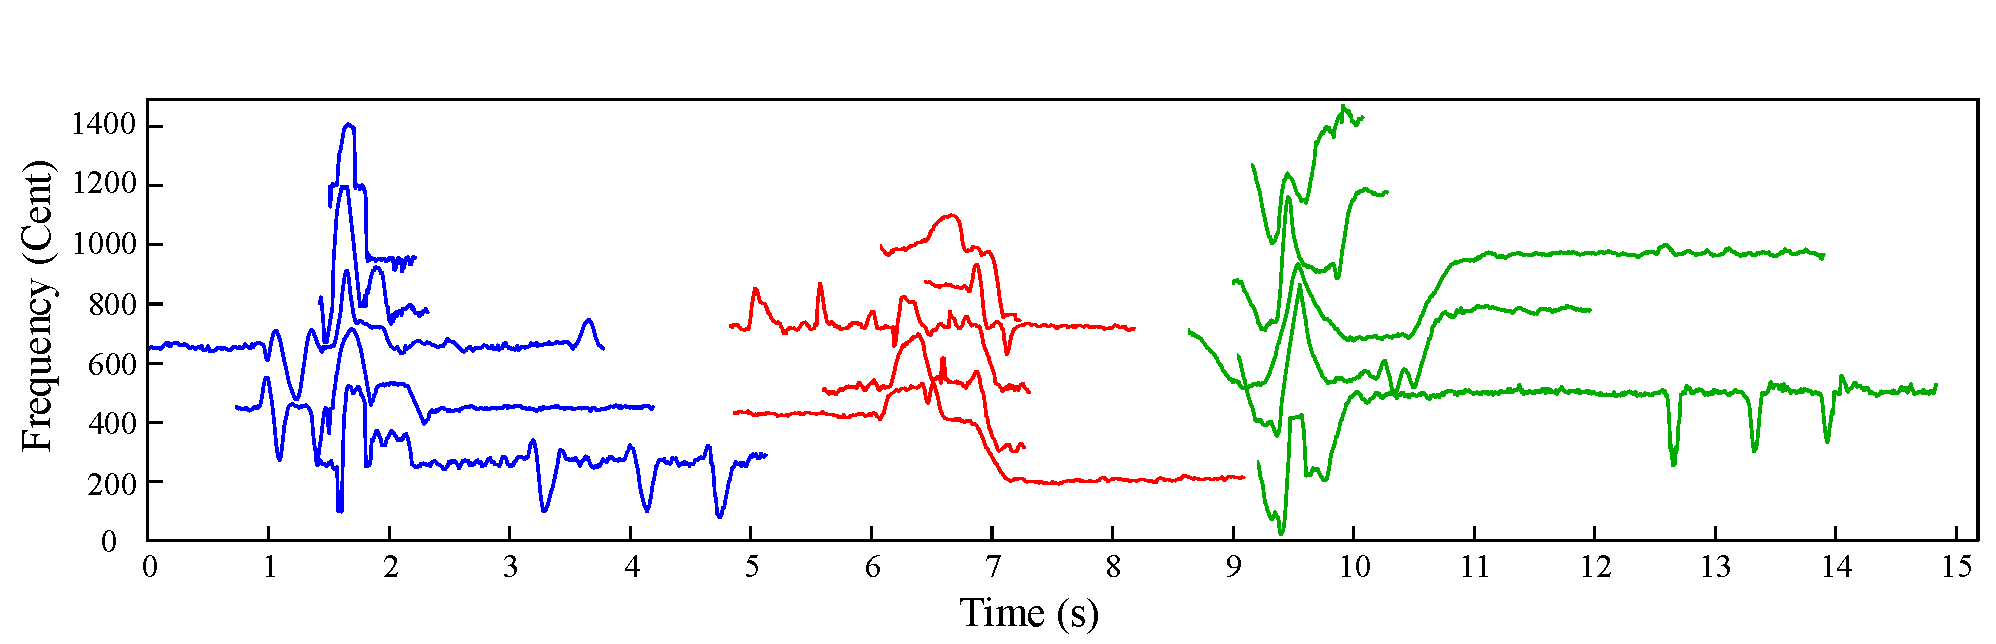
\includegraphics[width=\figSizeHundred]{ch01_introduction/figures/phraseClassesExample.pdf}
	\end{center}
	\caption{Pitch contours of occurrences of three different characteristic melodic phrases in Hindustani music. Contours are frequency transposed and time shifted for a better visualization.\TODO{diff aspect ratio?}}
	\label{fig:phraseComplexityExample_intro}
\end{figure}

An aspect that makes processing of melodies in \gls{iam} both interesting and challenging at the same time is the improvisatory nature of the music. The characteristic melodic phrases of \glspl{raga} (Section XX) act as the basis for artists to improvise, providing them with a medium to express creativity during \gls{raga} rendition. Since the essence of the music largely lies in the improvisatory aspects, artists bring in novelty through creatively transforming these melodic phrases as much as possible within the periphery defined by the \gls{raga} grammar. Therefore, the surface representation of these melodic phrases vary a lot across their occurrences. This high degree of variations in terms of the overall duration of a phrase, non-linear time warpings and the added melodic ornaments together pose a big challenge for melodic similarity computation and pattern extraction in \gls{iam}. In~\figref{phraseComplexityExample_intro} we illustrate this variability by showing the pitch contours of the different occurrences of three characteristic melodic phrases of the \gls{raga} Alaiya Bilawal. We can clearly see that the duration of a phrase across its occurrences varies a lot and the steady melodic regions are highly varied in terms of the duration and the presence of melodic ornaments. Thus, due to the improvisatory nature of the music, pattern processing in melodies of \gls{iam} becomes a challenging task. This context provides an opportunity to get deeper insights into the perception of melodic similarity and into the cultural influences on melodic similarity. 

Melodic characteristics in \gls{iam} differ significantly from a lot of other music traditions that are often the focus of studies in \gls{mir}. One peculiar characteristic of the melodies in Carnatic music (Section XX) is the meandering movement of the predominant pitch. Such melodic characteristics pose a challenge to melody transcription, a step often involved in the process of abstraction of melody. In addition, since these rapid pitch movements are characteristics aspect of melodic patterns they need to be preserved while computing melodic similarity, implying a fine grained representation of melody. Using a fine grained continuous predominant pitch representation of melody makes the task of pattern discovery further more difficult because of the computational complexity involved in the task.

%A beat level summarization of features, which is often performed in a number of tasks in \gls{MIR} to reduce the time-series dimensionality is not suited for melodies in \gls{iam}. 

%As mentioned, a composition mainly acts as a skeleton or a framework for an artist to construct a melody. In fact, typically the opening unmetered section, \gls{alap}, is not not based on any composition but is completely improvised. 

A vast majority of approaches for pattern processing in music focus on intra-opus or intra-recording pattern discovery. Since computational complexity is often one of the primary concerns in such a task, long duration of the performances in \gls{iam} pose a unique challenge. For long duration audio recordings lasting around an hour computational of self similarity becomes a computationally challenging task. To better understand the magnitude of computational complexity, consider a predominant pitch sequence of an hour long recording, sampled at 50\,Hz\footnote{a near-optimal sampling rate reported in \secref{sec:patterns_evaluation_of_similarity_measures}}. The pitch sequence comprises $1.8x10^{5}$ number of samples, which in turn amounts to nearly $3.2x10^{10}$ cells in the self similarity matrix. \XXX{S}{J}{Is this a strong point? how can we make it impressive} Thus, long performances in \gls{iam} introduce another set of challenges to this task. However, at the same time it is an opportunity as it provides a use-case to devise and test scalable approaches for pattern discovery from audio recordings. 


%Techniques that are typically employed to reduce the computational complexity in pattern processing task are; transcribe the melody to generate a symbolic score like representation and considering dimensionality reduced version of the feature, usually done through beat duration averaging. Applicability of both these techniques is questionable in the context of \gls{iam} owing the melodic characteristics. Melodic transcription is very complex and an ill defined task for melodic in \gls{iam}. And beat level summarization is musically not relevant since we are intersted in considering fine grained melodic nuances in the computation of melodic similarity. Moreover, estimation of beat locations is a  \TODO{complete it nicely}

\TODO{we are looking after really short duration patterns, that is also another challenge, please note that. Also typically beat summarization is done to reduce computational complexity, that can't be done here because 1) we wnt to present melodic nuances as the yare imp for simlarity and beat restimation is hard. Also for very small duration pattern that doesn't make sense....}


There is no standard frequency that is used as a reference for tuning instruments and voice in a music performances of \gls{iam}. The tonic pitch of the lead artist acts as the base frequency using which all the other instruments are tuned. Tonic pitch varies across artists and may vary across the different performance of an artist. In addition, an artist is free to choose any arbitrary frequency as a tonic in a performance. This aspect of music performance in \gls{iam} makes it difficult to directly compare melodies across different artists and audio recordings. 

There are many music traditions in the world where the manifestations of the seemingly transversal musical concepts such as melody and rhythm present a wide range of challenges to the current computational approaches in \gls{mir}. However, a very important factor behind selecting \gls{iam} for this analysis is the existence of musicological literature and well established music theory. \gls{iam} is an old music tradition whose origins can be traced back to the Vedas dating back to 1500 BCE. With that history, musical concepts in \gls{iam} are well studied and there exists a rich literature. This can be regarded as an opportunity, since basing the methodologies on the established music theories can speed up the advancements of computational approaches. 



%However at the same time not every computational task can directly benefit from the existing music theory. For example, the theory behind the concept of \gls{raga} in \gls{iam} elaborates WTF is happening to my mind!!!!!

%In this dissertation our focus is from an engineering perspective and solely on the computational aspects, we take established music theories for granted. Notably that is one major difference between an analysis like ours and studies in ethno-musicollogical. 


These challenges and opportunities offered by \gls{iam} sets in a unique context to develop novel methodologies for computational melodic anlaysis, and thus, improve the current state of the art in \gls{mir}. 






%
%\begin{itemize}
%	\item in general music similaity, search and discovery. Different applications and context
%	\item melodic analysis->representation of tonal content often used->melodic representaiton->difficulaty in extraction
%	\item problems which are solved by the state of the art in melody extraction for different music types
%	\item for which music types melodic anlaysis make more sense and have been done successfully.
%	\item Symbolic domain research, a lot of work.
%	\item Key detection and cover song detection.
%\end{itemize}
%
%\begin{itemize}
%	\item Music similarity focus in MIR
%	\item application and context of music similarity
%	\item how that has given rise to search and discovery in different contexts
%	\item use cases/ applications / relevant problems within similarity and search and discovery
%\end{itemize}

\section{Scope and Objectives}
\label{sec:intro_scope_context_relevance}

In this section we define the scope of our research work, clearly outline our objectives and enumerate the research questions addressed in this dissertation. 

Computational description and characterization of melodies is a broad research topic that can be approached from a number of perspectives involving different disciplines of science. In this dissertation we take a data-driven engineering approach and focus solely on the computational aspects of melodic analysis, building on top of the established music theories. Our applied research methodology, stands at an intersection of signal processing, machine learning and time-series analysis. We focus on content-based processing and the input data used in our approaches comprise audio recordings. The only exception to this is the approach described in~\secref{sec:patterns_characterization_of_melodic_patterns}, which utilize the associated editorial metadata of the recordings in addition to the audio data. The proposed approaches in this thesis are devised and evaluated on music collections in \gls{iam} that includes both Hindustani and Carnatic music. We now outline our broad objectives in this dissertation.

\begin{itemize}
%	\item To identify research tasks within computational melodic analysis that are relevant to \gls{iam}, and which can take advantage of the challenges and opportunities offered by this music tradition to improve the state of the art in \gls{mir}.
	\item To perform a critical review of the existing approaches in \gls{mir} relevant to our work in this dissertation.
	\item To build representative music corpora of \gls{iam} that comprises audio recordings and relevant editorial metadata, and use that to compile sizable and well annotated tests datasets for melodic analyses.
	\item To devise an approach to discover musically relevant melodic patterns in sizable audio collections of \gls{iam}
	\item To devise culture-aware and human interpretable approaches for automatic \gls{raga} recognition.
\end{itemize}


There are a number of research tasks within computational melodic analysis that are addressed in this dissertation (\figref{fig:tasks}), which sum up to achieve our broad objectives. Here we provide a brief description of these specific tasks, which also gives an idea about the evolution of the work done in this dissertation.

\begin{figure}[h]
	\begin{center}
		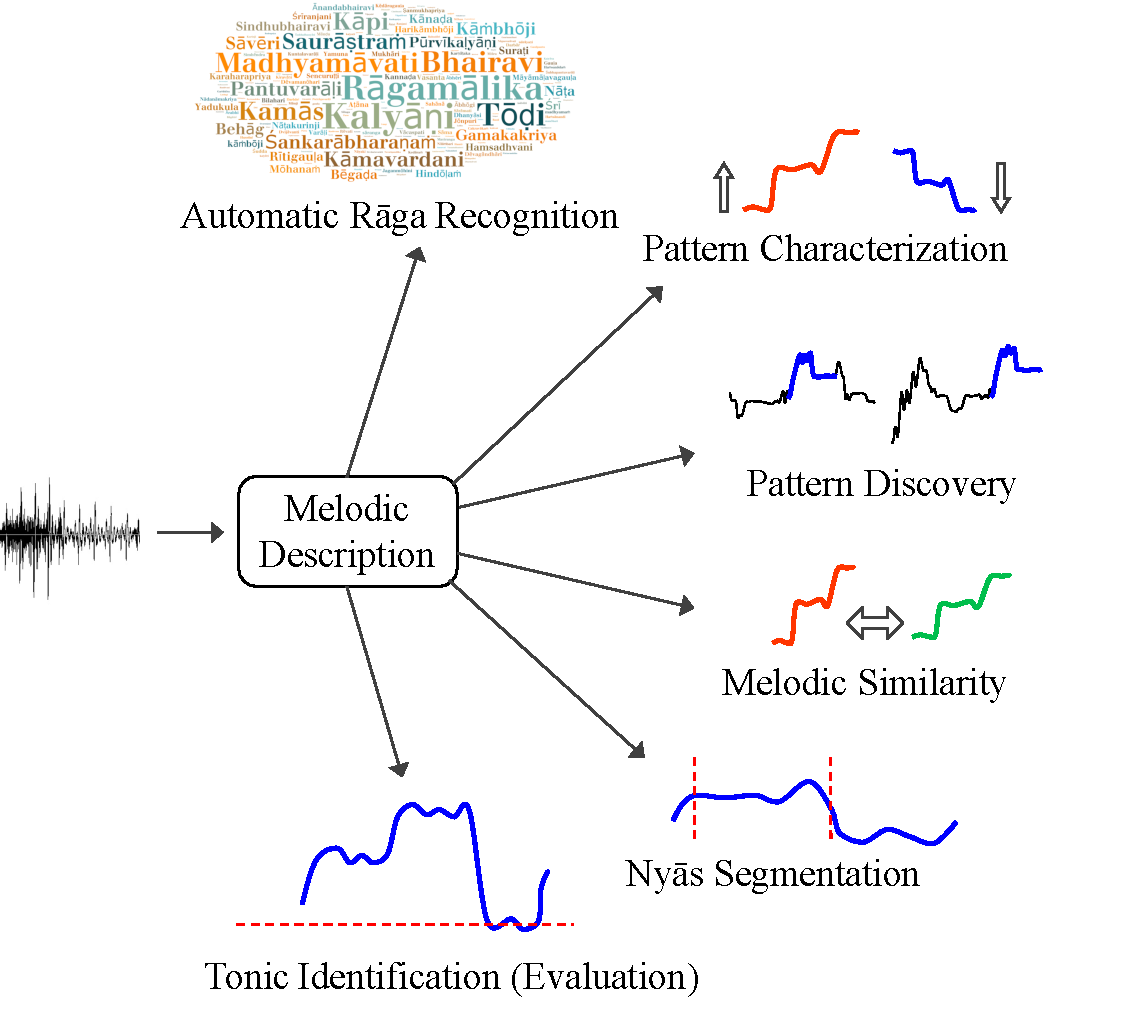
\includegraphics[width=\figSizeHundred]{ch01_introduction/figures/tasks.pdf}
	\end{center}
	\caption{Computational tasks within melodic analysis of \gls{iam} addressed in this dissertation.}
	\label{fig:tasks}
\end{figure}

As mentioned before, tonic pitch of the lead artist in a performance is the base frequency used for tuning by other instruments. For a meaningful comparison of melodies across artists and their recordings, identification of the tonic pitch in a recording is paramount. In recent past there are a number of methods proposed for tonic identification. However, a comparative evaluation of these methods on a common set of datasets is required to reach a consensus on the best performing method. We perform an extensive comparative evaluation of seven different tonic identification methods on six diverse datasets of \gls{iam} and identify the approaches that are robust and more accurate on both Hindustani and Carnatic music. In the process we also gain valuable insights into the types of errors made by tonic identification approaches, a useful information while devising methods that require tonic of the recordings as one of the inputs. 

Melody segmentation is a crucial step in pattern processing tasks, specifically in discovery of melodic patterns. Since \gls{nyas} \gls{svara} occurrences mark the boundaries of characteristic melodic phrases of \glspl{raga} in Hindustani music, detection of such segments becomes important for melodic segmentation. We therefore address the task of automatically segmenting \gls{nyas} \gls{svara} segments in the melodies of \gls{iam}.





\TODO{Objective of reproducible research, CompMusic philosophy}









we take an engineering perspective, MIR types approach of describing music, within and following CompMusic ideologies, culture specific in a multicultral context, applied, and micture of culture specific and 



\section{Organization and Outline of the thesis}
\label{sec:intro_organization}
